\documentclass[11pt,a4paper]{article}

  \usepackage[hmargin={25mm,25mm},vmargin={25mm,25mm}]{geometry}

  \usepackage{verbatim, ifpdf}
  \usepackage{graphicx, color}
  \usepackage{enumitem}

  \usepackage{amsmath}
  \usepackage{listings}
% \usepackage{enumerate}

% *********************************************************************
% The following lines should be ignored unless you know what you are
% doing, since the hyperref package is somewhat temperamental! 

  \IfFileExists{hyperref.sty}{%
    \ifpdf
      \usepackage[pdftex]{hyperref}
    \else
      \usepackage[dvips]{hyperref}
    \fi
    \definecolor{maroon}{RGB}{128,0,0}
    \hypersetup{pdfborder=0 0 0,colorlinks=true,plainpages=false,
                pageanchor=true,linkcolor=black,urlcolor=maroon}%
  }{%
    \providecommand{\url}[1]{\texttt{##1}}
    \providecommand{\href}[2]{##2\footnote{~See \texttt{##1}.}}%
  }

% End of hyperref setup.
% *********************************************************************

% The following optional parameters adjust paragraph spacing and
% indentation
  \setlength{\parskip}{1ex plus 0.5ex minus 0.2ex}
  \setlength{\parindent}{0pt}
  \addtolength{\skip\footins}{1.5 mm}

%%%%%  END OF PREAMBLE %%%%%%%%%%%%%%%%

%%%%%  THE MAIN TEXT STARTS HERE %%%%%%

\begin{document}

\vspace*{\fill}
\begin{center}
\textbf{{\huge $L_1$ Optimisation and Regularisation}}
\end{center}
\vspace*{\fill}
\pagebreak

\section{Basis Pursuit}
In signal processing, we have a signal $\mathbf{s}$ and we want to fit it to a basis of waveforms, such as the Fourier matrix for Fourier transforms, or other wavelet patterns. This gives rise to the problem
\begin{center} $\Phi \mathbf{\alpha} = \mathbf{s}$ \end{center}
where $\Phi$ is the waveform matrix and $\mathbf{\alpha}$ is the decomposition of the signal. \\
In the case where the signal is coarse, i.e. there are more parameters than variables, there are multiple solutions of $\mathbf{\alpha}$ that would fit the data. One way to choose the solution is to minimise $||\alpha||_1$. This method is called \textbf{basis pursuit} because, as we shall see, it restricts the number of waveform vectors used in the decomposition. This is different to other methods, such as minimising $||\alpha||_2$. \\
\subsection{Equivalence to linear programming}
We can rewrite the problem as a linear program as follows: \\
Set $A = \begin{pmatrix} \Phi & \text{-}\Phi \end{pmatrix}$, $\mathbf{x} = \begin{pmatrix} \alpha_1^+ & \alpha_2^+ & ... & \alpha_m^+ &  \alpha_1^- & \alpha_2^- & ... & \alpha_m^- \end{pmatrix}^T$, $\mathbf{b} = \mathbf{s}$, $\mathbf{c} = \mathbf{1}$, where $x^+ = max(x,0)$, $x^- = max(0,-x)$. \\
Then the problem of basis pursuit becomes the conventional linear programming problem of min $\mathbf{c}^T\mathbf{x}$ subject to $A\mathbf{x} = \mathbf{b}$. This can be solved by the simplex algorithm or interior point methods. \\

Note that a corollary of this method is that, since the solution to a linear programming problem lies on an extreme point, we would have at most n nonzero entries in $\mathbf{x}$, where n is the number of nonzero entries in the signal. In this way, if the system is highly overdetermined, the result will still be sparse (and hence can be stored with less memory). Also, we are effect finding a suitable basis of waveform vectors and representing the signal in this basis, hence the name basis pursuit. \\

\textbf{I don't really understand this.} \\

\section{Basis Pursuit with Noise}
We may want to allow some noise in the signal, i.e. we don't force $\Phi \mathbf{\alpha} = \mathbf{s}$. Instead, we change the objective function to
\begin{center} $||\Phi \mathbf{\alpha} - \mathbf{s}||_2^2 + \lambda ||\alpha||_1$ \end{center}
for some constant $\lambda$. (Why do we take the Euclidean norm of the first term rather than $L_1$ norm?) This is now equivalent to the linear regression problem with $L_1$ regularisation. \\

First, we show that this is equivalent to ordinary least squares regression with a constraint on the $L_1$ norm (note the change of variables):
\begin{center} min $||X\mathbf{\beta} - \mathbf{Y}||_2^2$ subject to $||\mathbf{\beta}||_1 \leq t$. \end{center}
This is because we can use Lagrange multipliers with the slack variable $\mathbf{z}$ where
\begin{center}
	$L(\mathbf{\beta}, \mathbf{\lambda}) = ||X\mathbf{\beta} - \mathbf{Y}||_2^2 + \mathbf{\lambda_1}^T(\sum \mathbf{\beta} + \mathbf{z_1} - t) + \mathbf{\lambda_2}^T(-\sum \mathbf{\beta} - \mathbf{z_2} + t)$ \end{center}
This has the same gradient conditions as the basis pursuit with noise problem, and we can find $\lambda_1$, $\lambda_2$ which are feasible in the constrained problem to satisfy the conditions. Hence the two problems are the same. \\

\subsection{Investigation on Diabetes Dataset}
We look at the LASSO method on a toy dataset, and compare it to ordinary least squares and other normalisation methods. The dataset records a quantitative measure of diabetes progression with features including age, sex, BMI, blood pressure, and six blood serum measurements. \\

We now look at the graph of coefficients as we adjust the $\lambda$ factor in the $L_1$ regularisation term. Note that the coefficients are piecewise linear. This is because if we compute the partial derivatives, we get
\begin{center} $\mathbf{\beta} = (X^TX)^{-1} (X^TY \mp \mathbf{\lambda})$ \end{center}
where the plus and minus are the opposite of the sign of $\mathbf{\beta}$. So, locally, as we increase $\mathbf{\lambda}$, the coefficients decrease linearly, and the factor changes when one of the coefficient changes sign (i.e. becomes 0). As we can see from the figure, as we increase the value of $\mathbf{\lambda}$, more and more coefficients are set to 0. This reduces the number of independent variables and helps with the interpretation. In this case, 's5' and 'bmi' are more relevant for measuring diabetes progression than some of the other features, such as 's1' and 's2'. The reason why it favours some coefficients being set to 0 is as follows: at the linear stage, we can find a $\mathbf{\lambda_0}$ such that $\mathbf{\beta_j} = 0$. What happens after that? Well, if we want to change $\mathbf{\beta_j}$, then we would change the squared error by the same amount as we did before. However, since $\mathbf{\lambda}$ is now larger, it would change the $L_1$ norm by more than before. So it is not worth changing the coefficient to a different value. Since the coefficients are continuous in $\mathbf{\lambda}$, we would have $\mathbf{\beta_j} = 0$ for all $\mathbf{\lambda} > \mathbf{\lambda_0}$. \\

\begin{figure}[htbp]\centering\label{fig1}
  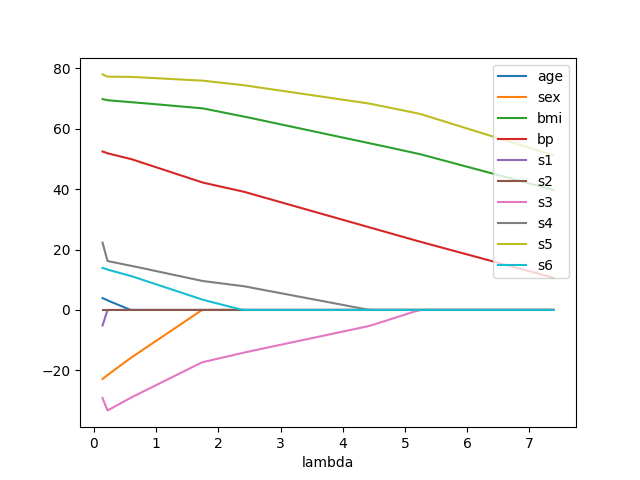
\includegraphics[height=78mm,angle=0]{fig1.png}
  \caption{Values of coefficients in LASSO regression for different values of $\lambda$.}
\end{figure}

We can also look at the train and test $R^2$ values. Here, we compare the three methods: OLS, LASSO and Ridge regression ($L_2$ normalisation). As expected, the test value is lower than the train value, because there is always some degree of overfitting to the training data. Although train $R^2$ decreases as we increase $\mathbf{\lambda}$, the test $R^2$ can be higher than that for the OLS (although only slightly). This shows that in some cases, LASSO is helpful in reducing overfitting. Also, normalisation helps in reducing the volatility of the test $R^2$ compared to OLS. Finally, note that the same coefficient of $\mathbf{\lambda}$ has a more significant effect for LASSO compared to Ridge. This is because the coefficients are small (probably) so LASSO gives a larger penalty than Ridge. \\

\begin{figure}[htbp]\centering\label{fig2}
  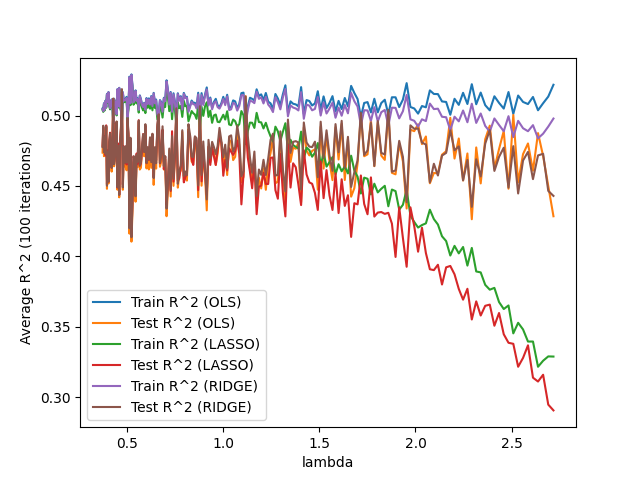
\includegraphics[height=78mm,angle=0]{fig2.png}
  \caption{Train and test $R^2$ values in LASSO and Ridge regression for different values of $\lambda$.}
\end{figure}

\section{Regularisation in neural networks}
Neural networks are a very popular machine learning algorithm. They work as follows: we have input data $\mathbf{x}_0$, and our model is as follows:
\begin{align*}
\mathbf{x}_1 &= \sigma(A_1 \mathbf{x}_0 + \mathbf{b}_1) \\
\mathbf{x}_2 &= \sigma(A_2 \mathbf{x}_1 + \mathbf{b}_2) \\
&... \\
\mathbf{x}_n &= \sigma(A_n \mathbf{x}_{n-1} + \mathbf{b}_n) \\
\end{align*}
$\mathbf{x}_n$ is the output. Here, the As are matrices of parameters, the bs are the bias parameters, and $\sigma$ is a non-linear function, for example ReLU: $\sigma(x) = max(x,0)$. This type of model is very expressive and can accurately represent a wide range of functions (compared to linear regression). \\

To find the "best" parameters A and b, we construct a loss function, and use numerical methods to find the parameters which minimise this loss function. For categorical prediction problems, typically the loss function would be cross-entropy loss: where $\mathbf{x}_n$ is the vector of probabilities for each class, we would have $loss = L = -log(\mathbf{x}_n^{(y)})$, where y is the correct value. (and obviously add it across all samples). \\

As for the method to find the parameters, we typically use variants of stochastic gradient descent. This is where we take a small batch of the sample data, and change the parameters in the direction of the gradient of the loss function: 
\begin{center} $A_i = A_i - \lambda \frac{\partial L(x_1, ..., x_m)}{\partial A_i}$ \end{center}
where $x_1, ..., x_m$ is the batch of data, and $\lambda$ is a learning rate. The reason why we only take a small batch is that each step would take too long if we do gradient descent on the whole dataset. Moreover, this also helps reduce overfitting. This is because neural networks have many more parameters than data, so they are extremely prone to overfitting. By only looking at the gradient of a small sample (and a different sample each time), we would not reach a point where the neural network is perfect on each of the training datum, but instead only learn the parts which prevail in most of the training set. \\

Since neural networks are prone to overfitting, we may wish to introduce regularisation to this problem. This would work in the same way as linear regression above: we tweak the loss function such that
\begin{center} $L = L + \lambda_1 \sum_i |A_i|$ \end{center}
or 
\begin{center} $L = L + \frac{\lambda_2}{2} \sum_i A_i^2$ \end{center}
where $A_i$ are the parameters. ($L_1$ and $L_2$ regularisation respectively). The way to incorporate this in the training process is simple. In PyTorch, there is a parameter \emph{weight\_decay} for the optimiser which multiplies the weight by a fixed factor every time we run SGD. This coincides with $L_2$ regularisation, because the gradient of the regularisation term is precisely $\frac{\partial L}{\partial A_i} = \lambda_2 A_i$. As for $L_1$ regularisation, we can manually change the gradient function by the gradient of the regularisation term, which is $\lambda_1 sign(A_i)$.

\subsection{Investigation on GTSRB dataset}
To get a sense of how this impacts the training of neural networks, we implement $L_1$ and $L_2$ regularisation on the German Traffic Sign Recognition Benchmark dataset. This is a dataset of around 50000 images, with the task being to classify these images into 43 different traffic signs. We use the LeNet architecture on this problem, which is a basic architecture with a few convolutional layers and max pool layers, followed by a few fully connected layers. (We do not go into details of neural network architecture here.) We trained the network for 15 epochs (i.e. going through the training set 15 times). This took around 10 minutes on Google Colab with the free GPU. Since the training time is not short, we could not train the network for a large number of values of $\lambda_1$ and $\lambda_2$ and plot graphs. Instead, we train 3 networks, one without regularisation, one with $\lambda_1 = 10^{-5}$, and one with $\lambda_2 = 10^{-4}$. The learning rate used here is a constant $10^{-3}$ throughout. \\

We first look at two metrics for the 3 networks: accuracy and loss.
\begin{figure}[htbp]\centering\label{fig3}
  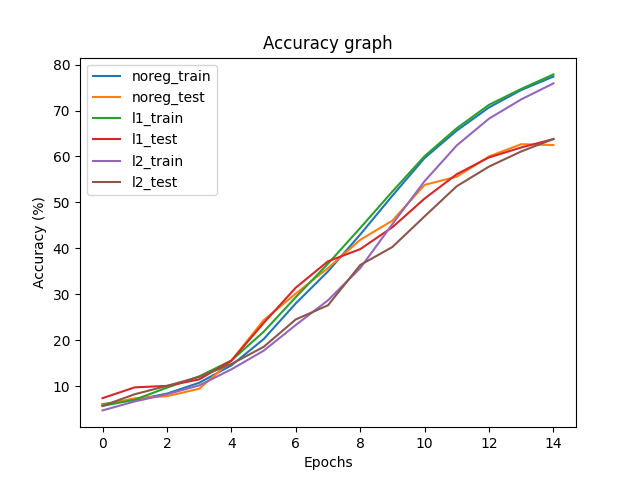
\includegraphics[height=78mm,angle=0]{fig3.png}
  \caption{Train and test accuracy values in neural networks.}
\end{figure}
\begin{figure}[htbp]\centering\label{fig4}
  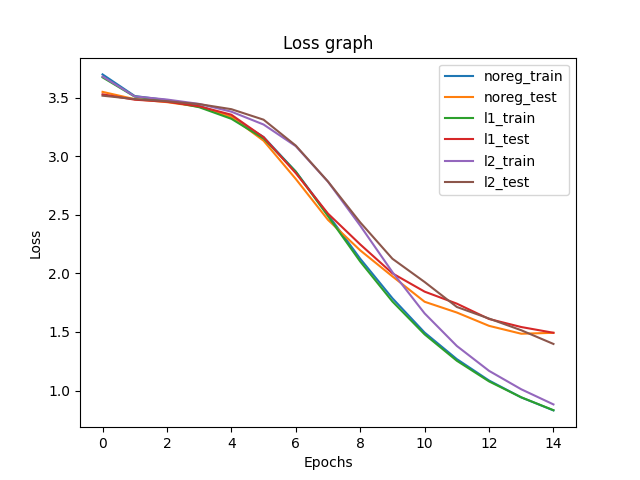
\includegraphics[height=78mm,angle=0]{fig4.png}
  \caption{Train and test loss values in neural networks.}
\end{figure}

Notice that the graphs for $L_1$ and no regularisation are quite similar, while that for $L_2$ lags slightly behind. This may be because we chose too large a coefficient for the $L_2$ regularisation. Also, there is almost no difference between test and train loss/accuracy in the first 7 epochs, with the gap beginning to widen in later epochs. The gap did not seem to be smaller for the $L_1$ and $L_2$ regularisation cases, although there seemed to be some difference in the last epoch. Perhaps we should run the training for longer to get a better idea of what is happening.

Also, we may expect that as in linear regression, using $L_1$ regularisation means some of the parameters will be set to zero. We do not observe this in the case of neural networks. This is because of the way we approach the problem -- under SGD, even if we turn $\lambda_1$ to be large, we would only get the coefficient oscillating around 0 since the $L_1$ gradient term dominates. But even this is not the case. So $L_1$ regularisation probably loses the advantage of interpretability in a neural network setting. \\



\end{document}